\chapter{Tasks Assigned}
\label{chap:tasks}

% [Detailed explanation of your methodology, code, and
%  problem-solving — this should be the longest section]

\section{Wireframing and UI Design}

A significant portion of the internship was dedicated to UI/UX design for the GeneSolutions pregnancy mobile application. The project required designing the interfaces for three distinct features: a Baby Naming tool, an After Birth tracking suite, and an internal Admin Portal. All three were delivered through a consistent iterative workflow — translating written requirements into screen designs, gathering client feedback, and refining until a prototype was ready for demo.

\subsection{Design Workflow}

The design process for each screen followed a consistent three-stage pipeline. First, the functional requirements for the screen were reviewed and distilled into a structured prompt, which was used either with Google Stitch AI or directly in VS Code using React and TypeScript via an AI-assisted vibe-coding approach to generate a first-draft layout. This initial draft served as a low-effort starting point rather than a blank canvas, allowing rapid exploration of layout options. Second, the generated screens were imported and arranged on a Figma or FigJam board, where navigation flows, button logic, and screen transitions were mapped out and refined. Third, the resulting prototype was reviewed by the client in sessions held approximately two to three times per week. Early review cycles focused primarily on high-level flow and structure, while later rounds narrowed to finer details such as label wording, component spacing, and interaction states. This iterative loop continued for approximately three weeks until a stable prototype was approved for handoff to the development team.

\subsection{Baby Naming Tool}

The Baby Naming tool is a personalised name recommendation feature that combines Numerology and Feng Shui to help expecting mothers find a meaningful name for their child. The designed screens covered the full user flow across six stages.

The entry screen allows mothers to select their preferred naming method — Numerology (based on birth date) or Feng Shui (based on birth year and elemental destiny). A detailed input form then collects the baby's gender, the family surname, the mother's preferred naming style, the expected or actual birth date, and a dropdown of blessings or character traits the mother wishes for her child.

Following submission, the app generates a curated list of name suggestions with a brief summary visible inline and a full analytical breakdown accessible on tap. A history log screen allows mothers to revisit previously generated lists. The deep analytics view presents a four-part breakdown of the selected name, covering the linguistic and emotional story behind the name, a Pythagoras birth chart decoding, an integrated name-and-birth-date compatibility grid, and personalised parenting insights derived from the child's numerology profile. Finally, a shareable ``Certificate of Love'' screen was designed to allow mothers to export and share a visual keepsake of the baby's name and its meaning to social platforms. The complete screen flow is illustrated in Figure~\ref{fig:babynaming}.

\begin{figure}[h]
    \centering
    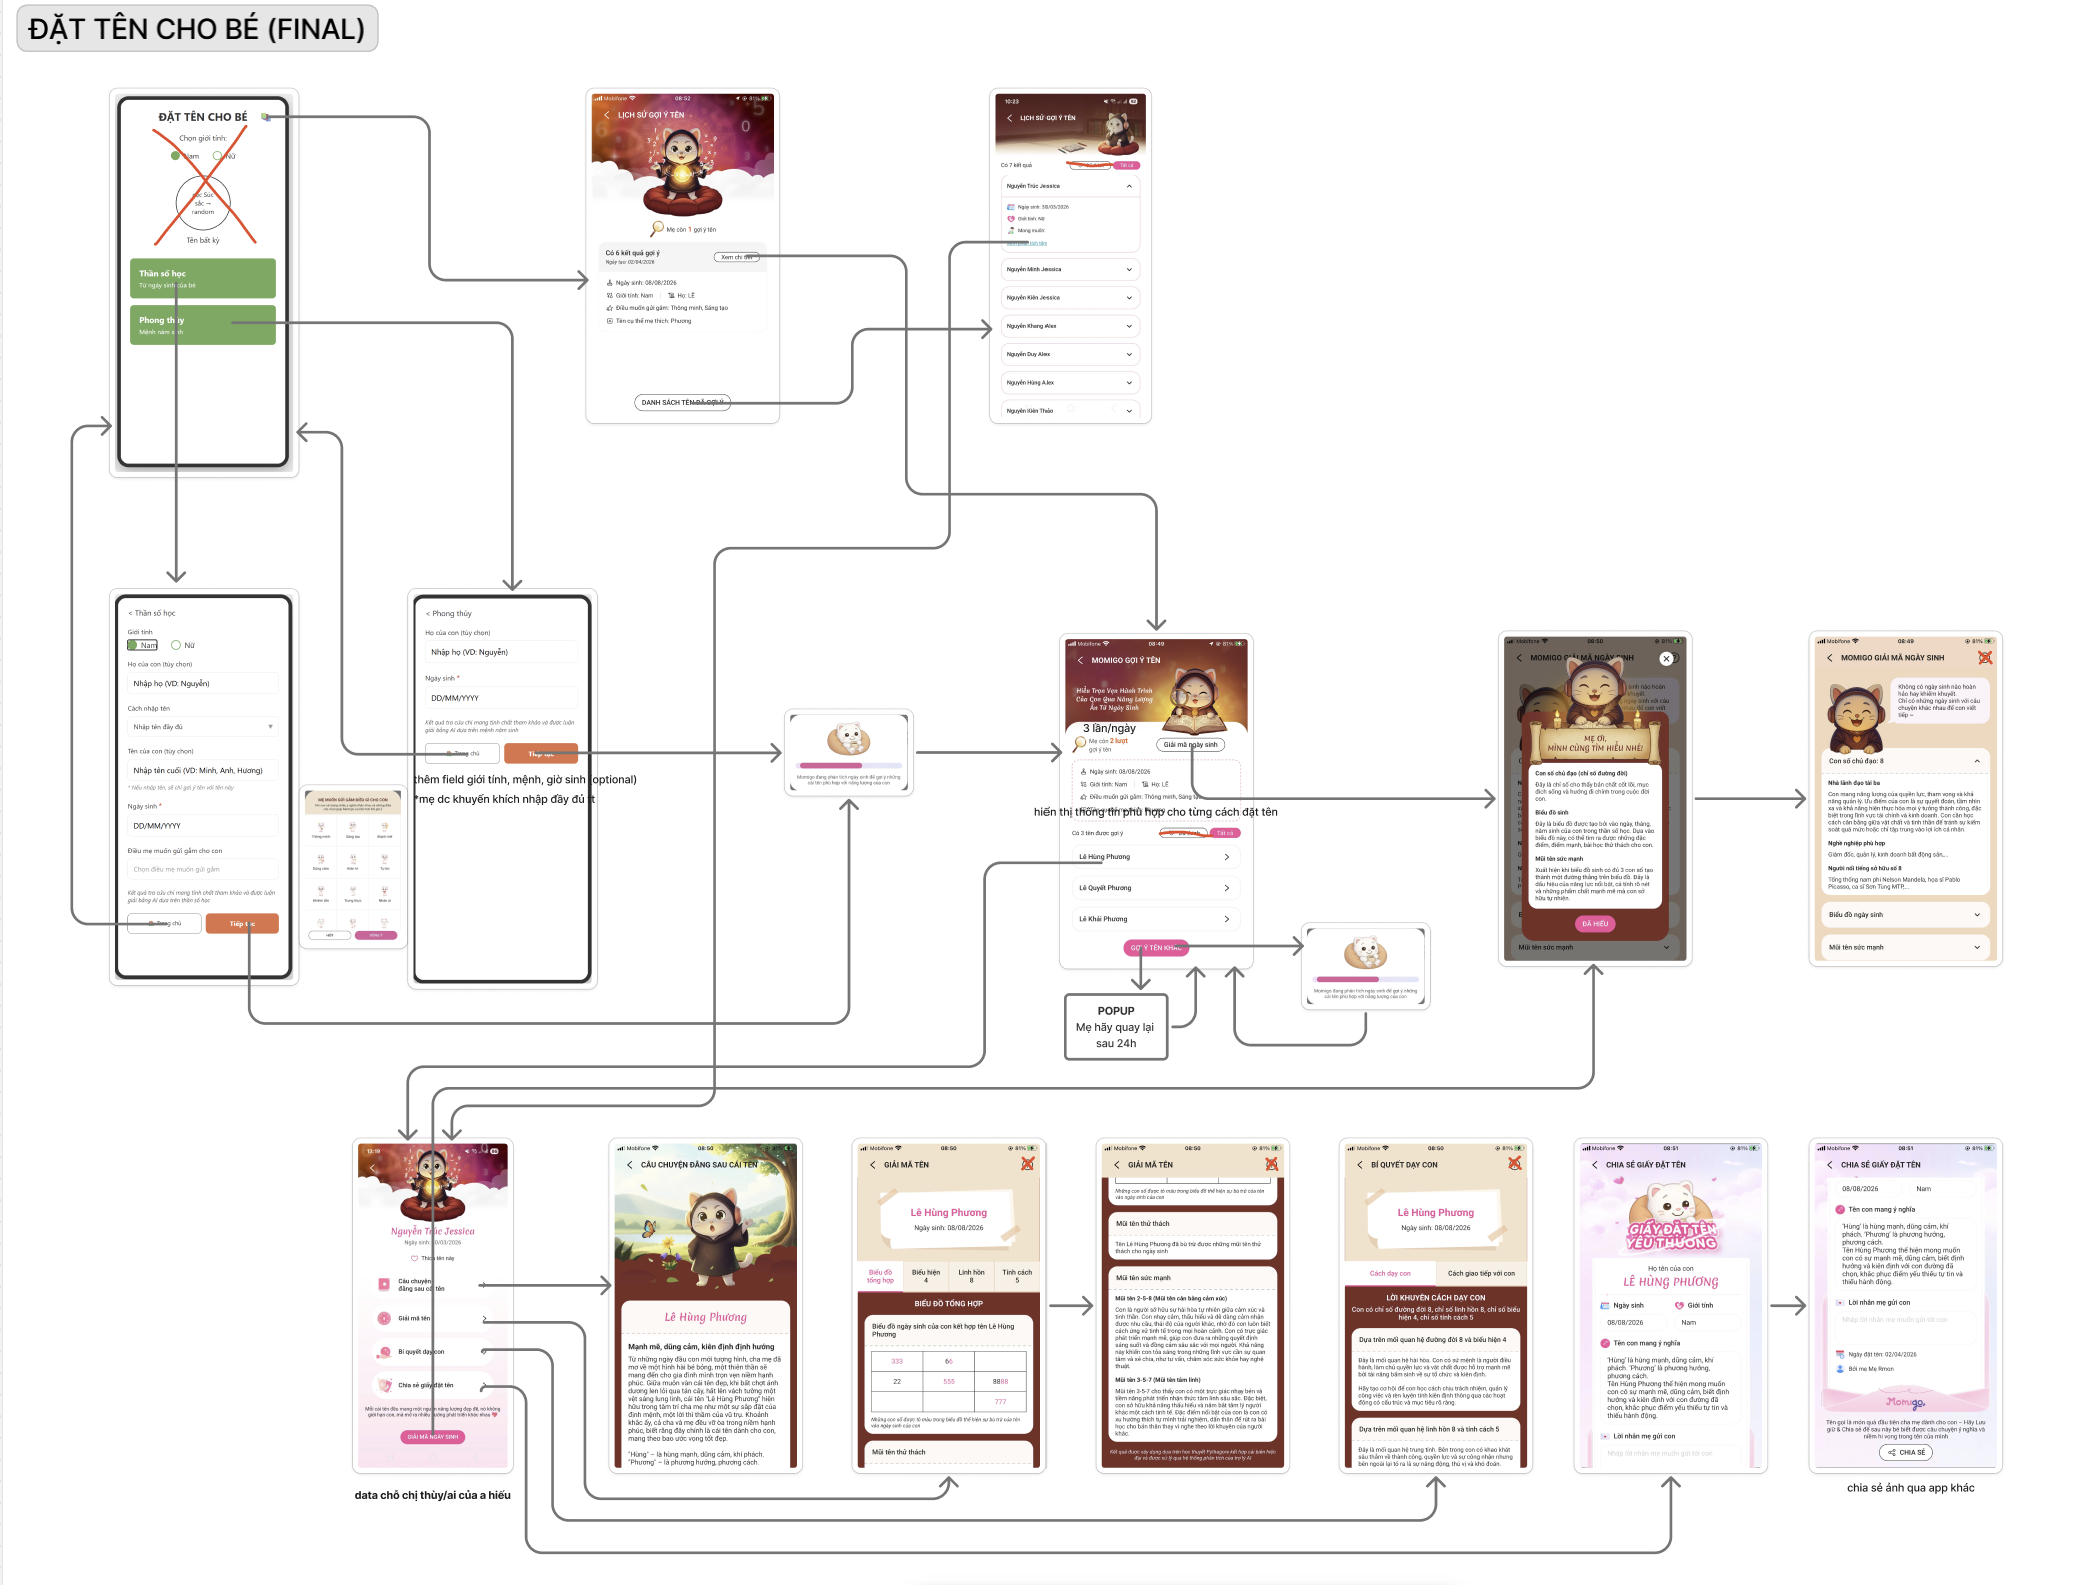
\includegraphics[width=0.8\textwidth]{img/baby_naming_tool.png}
    \caption{FigJam flow diagram for the Baby Naming tool. \href{https://www.figma.com/board/HeyvaGyDvu1yq7RaZO9zRI/Untitled?node-id=0-1&t=ZxCfVuSMaxPwvhv0-1}{Click here to view the interactive FigJam board.}}
    \label{fig:babynaming}
\end{figure}

\subsection{After Birth Suite}

The After Birth suite activates dynamically once a mother records that she has given birth. At 41 weeks of pregnancy, a pop-up prompts the mother to confirm delivery, which triggers a transition from prenatal tracking mode into a postpartum dashboard personalised to the newborn.

The onboarding flow guides the mother through setting up the baby's profile — uploading a photo, entering the full name, gender, birth date and time, and initial weight and height measurements. The central dashboard provides a real-time health summary showing the baby's exact age in months and days, the next upcoming vaccination with a countdown, and the latest growth snapshot with delta indicators from the previous entry. A multi-child management screen was also designed to allow mothers to switch between profiles for multiple children.

The Growth Tracking module features interactive weight and height charts plotted over a monthly timeline, with WHO growth standard benchmarks overlaid to automatically classify the baby's development as within the normal range or flagged as below average. An entry form allows new measurements to be logged by date, with an auto-generated quick analysis summary.

The Immunisation Scheduler organises all required vaccines month by month, explicitly naming each critical shot — including Hepatitis B, the 5-in-1 Quinvaxem/Pentaxim, Rotavirus, Pneumococcal, etc. — to ensure no doses are missed. Finally, the Milestone Journal provides a visual timeline feed where mothers can log dated entries with photos and videos, categorised by milestone type, health events, or sleep records. The full postpartum flow is illustrated in Figure~\ref{fig:afterbirth}.

\begin{figure}[h]
    \centering
    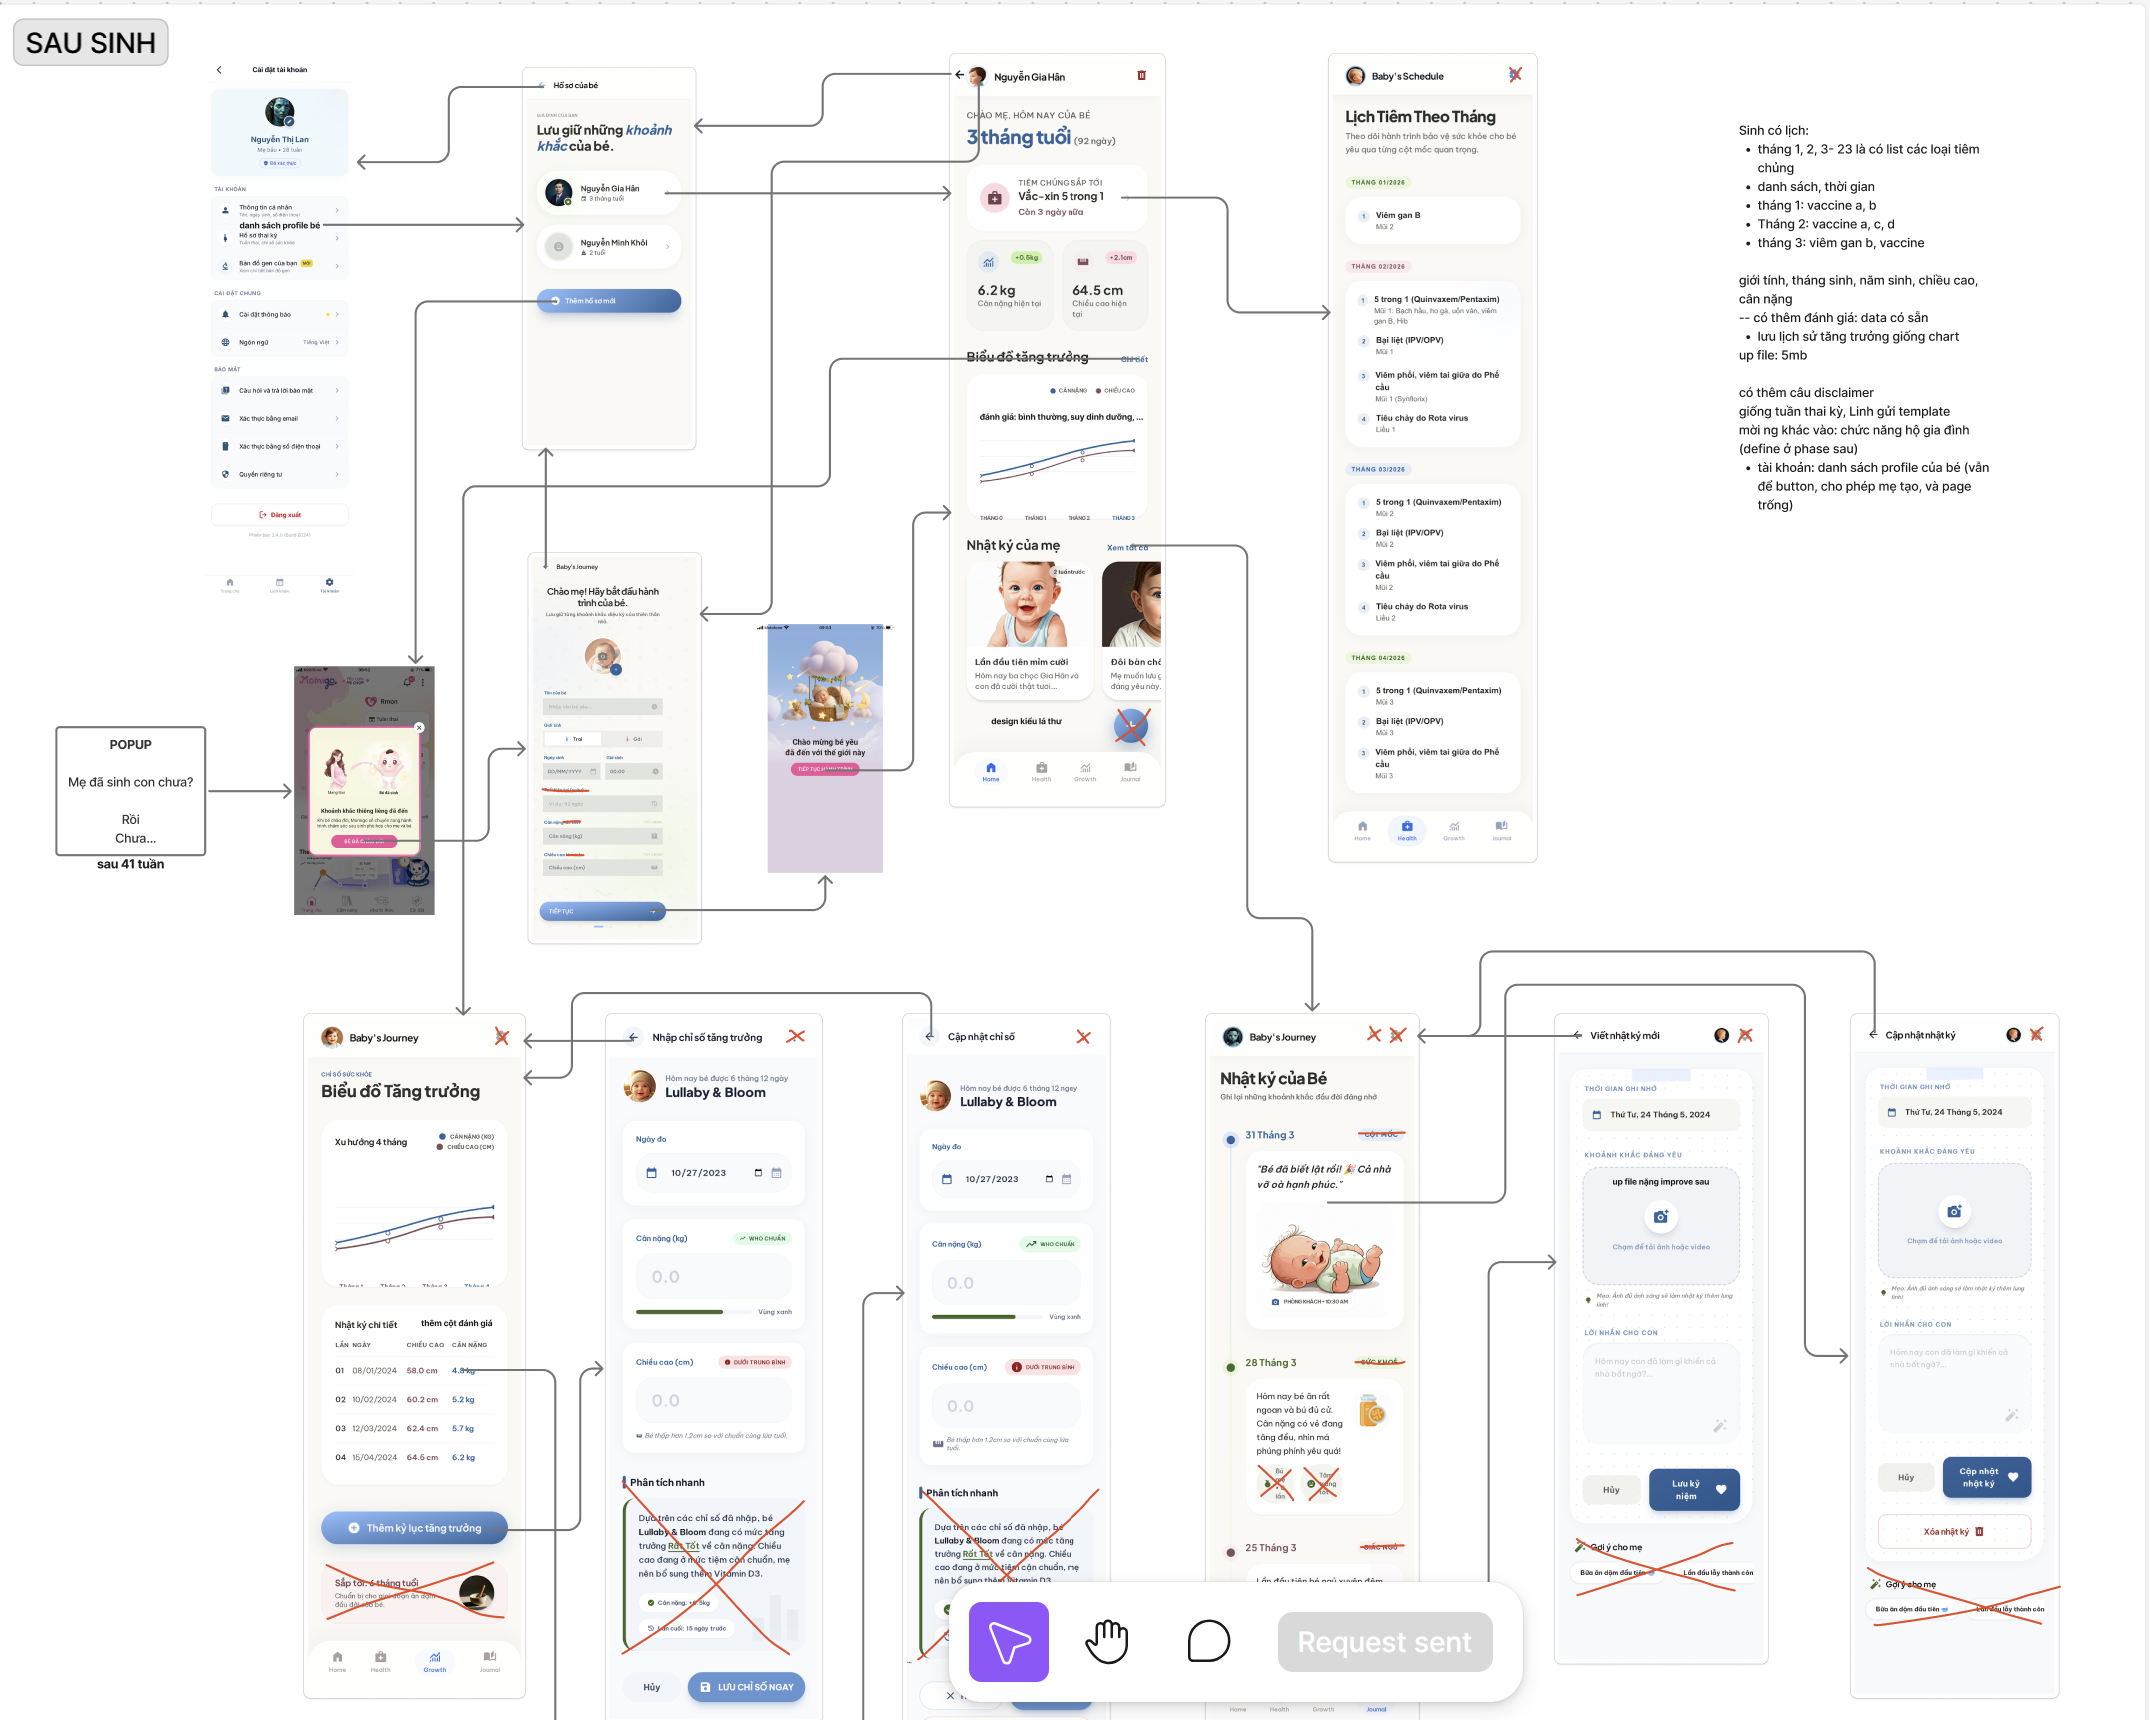
\includegraphics[width=0.8\textwidth]{img/after_birth_tool.png}
    \caption{FigJam flow diagram for the After Birth suite. \href{https://www.figma.com/board/HeyvaGyDvu1yq7RaZO9zRI/Untitled?node-id=0-1&t=ZxCfVuSMaxPwvhv0-1}{Click here to view the interactive FigJam board.}}
    \label{fig:afterbirth}
\end{figure}

\subsection{Admin Portal}

The Admin Portal is a web-based Content Management System (CMS) designed for use by the GeneSolutions operations and marketing team. It provides centralised control over all content, media, clinical surveys, and user accounts within the mobile application — removing the dependency on software releases for routine content updates.

The portal's authentication screen provides a secure login entry point restricted to credentialled GeneSolutions staff. Upon login, a welcome dashboard greets the administrator and defers detailed analytics to a future release phase.

The Handbook Management module supports two content pipelines: native article creation, where admins write and publish articles from scratch using a rich text editor with category and author assignment; and Sale Portal fetching, which pulls pre-vetted corporate content from a linked business platform. Fetched articles have their core fields permanently locked to protect brand and medical accuracy, with admins only permitted to configure app-specific metadata such as categories and target pregnancy stage tags.

The Media Library module covers three sub-sections: banner management with drag-and-drop reordering, a general photo asset repository, and a theming dashboard for applying visual templates across the application.

The Clinical Checklist module provides a form builder interface for creating and versioning clinical surveys, with per-step and per-field configuration including field type, validation rules, and optional or mandatory toggles. 

Finally, the User and Admin Access Control module maintains separate registries for admin accounts and end-user accounts, with a detailed per-user view exposing account metadata and synchronised health parameters such as weight, height, blood type, and current pregnancy week. The portal flow is illustrated in Figure~\ref{fig:adminportal}.

\begin{figure}[h]
    \centering
    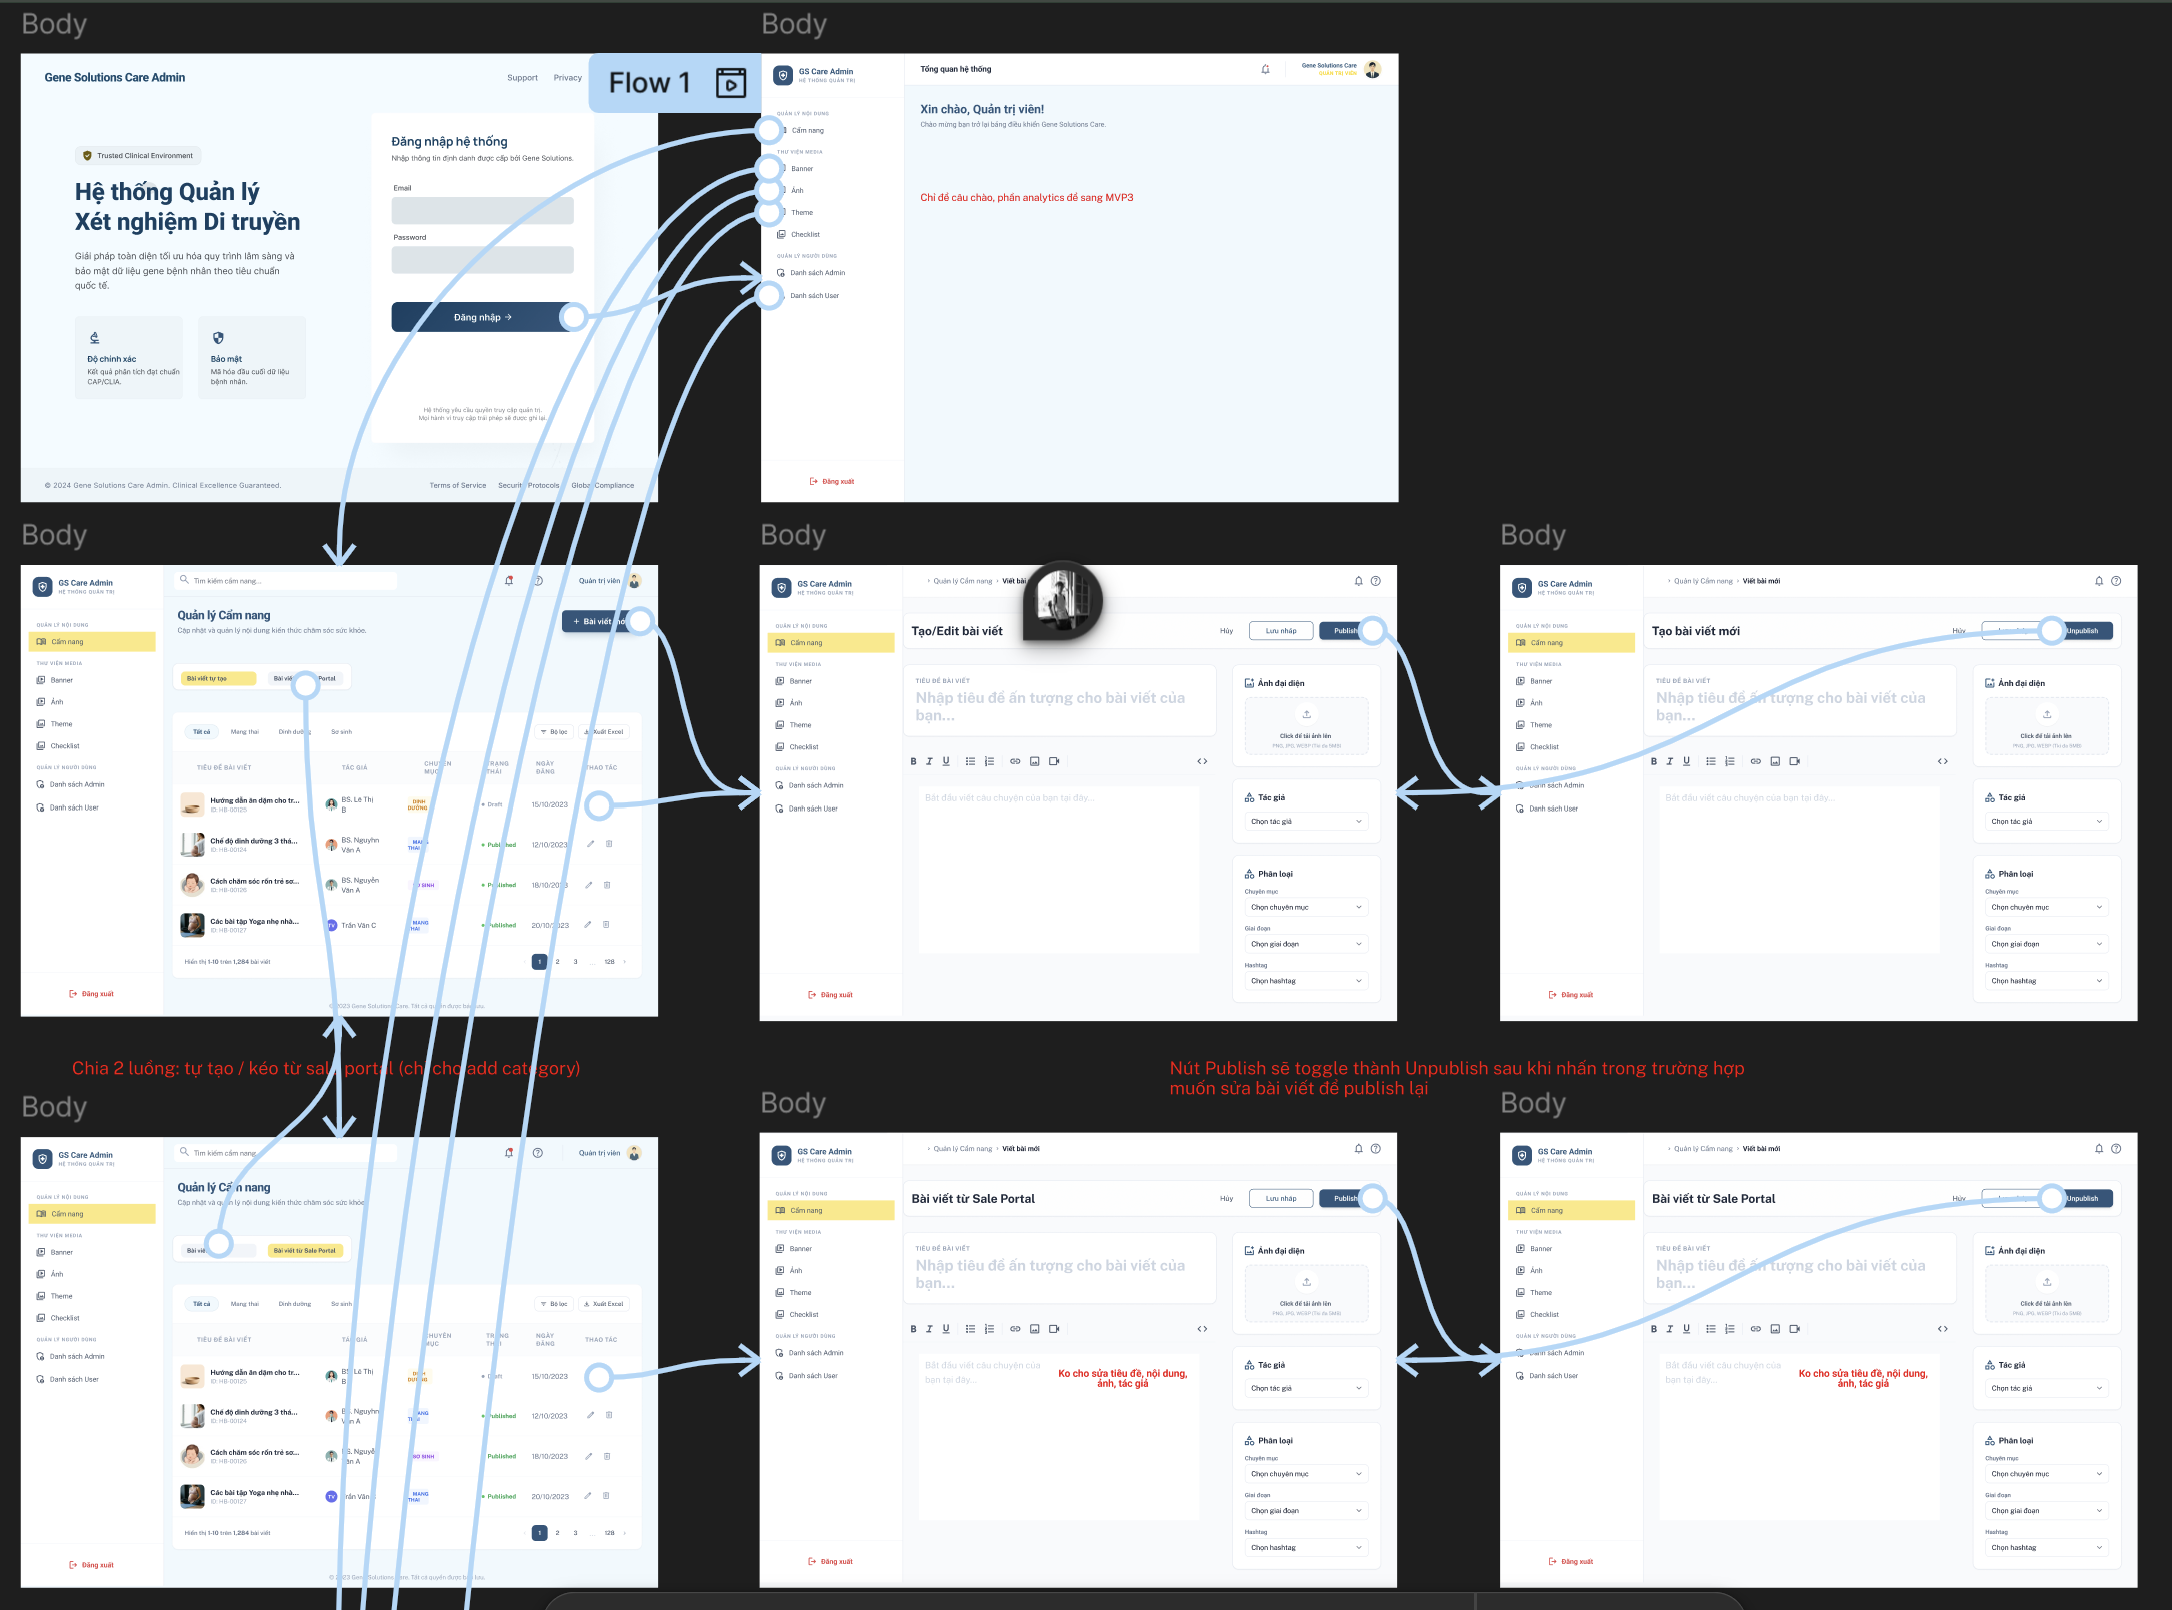
\includegraphics[width=0.8\textwidth]{img/admin_portal.png}
    \caption{FigJam flow diagram for the GS Care Admin Portal. \href{https://www.figma.com/design/D2IvIy9szuOS218QLGbgGk/admin-portal-wireframe?node-id=0-1&t=yZhukm96npUyIkCy-1}{Click here to view the interactive Figma wireframe.}}
    \label{fig:adminportal}
\end{figure}

\section{Project Management}

Project management was a core responsibility throughout the internship, spanning five concurrent projects: Masan, Syngenta, P\&G, INNOVA US, and GeneSolutions. The primary tools were Azure DevOps Boards for sprint planning and task tracking, Microsoft Teams for meeting coordination, and Microsoft Excel for supplementary tracking of timelines, deadlines, and ownership.

\subsection{Sprint Planning on Azure DevOps}

Each project was managed through one-week sprints on Azure DevOps Boards. At the start of each sprint, tasks were created and broken down into smaller subtasks, each assigned a deadline, a person in charge, and a status label. A typical sprint board carried five to six high-level tasks spanning all roles — Business Analysis, Quality Control, and multiple development tracks — with each task decomposed into several subtasks to reflect the actual unit of daily work. Across the five active projects, this amounted to coordinating task assignment and progress tracking for a team of approximately 15 people, including 8 developers. Figure~\ref{fig:sprintboard} shows a sample sprint board for the Masan project.

\begin{figure}[h]
    \centering
    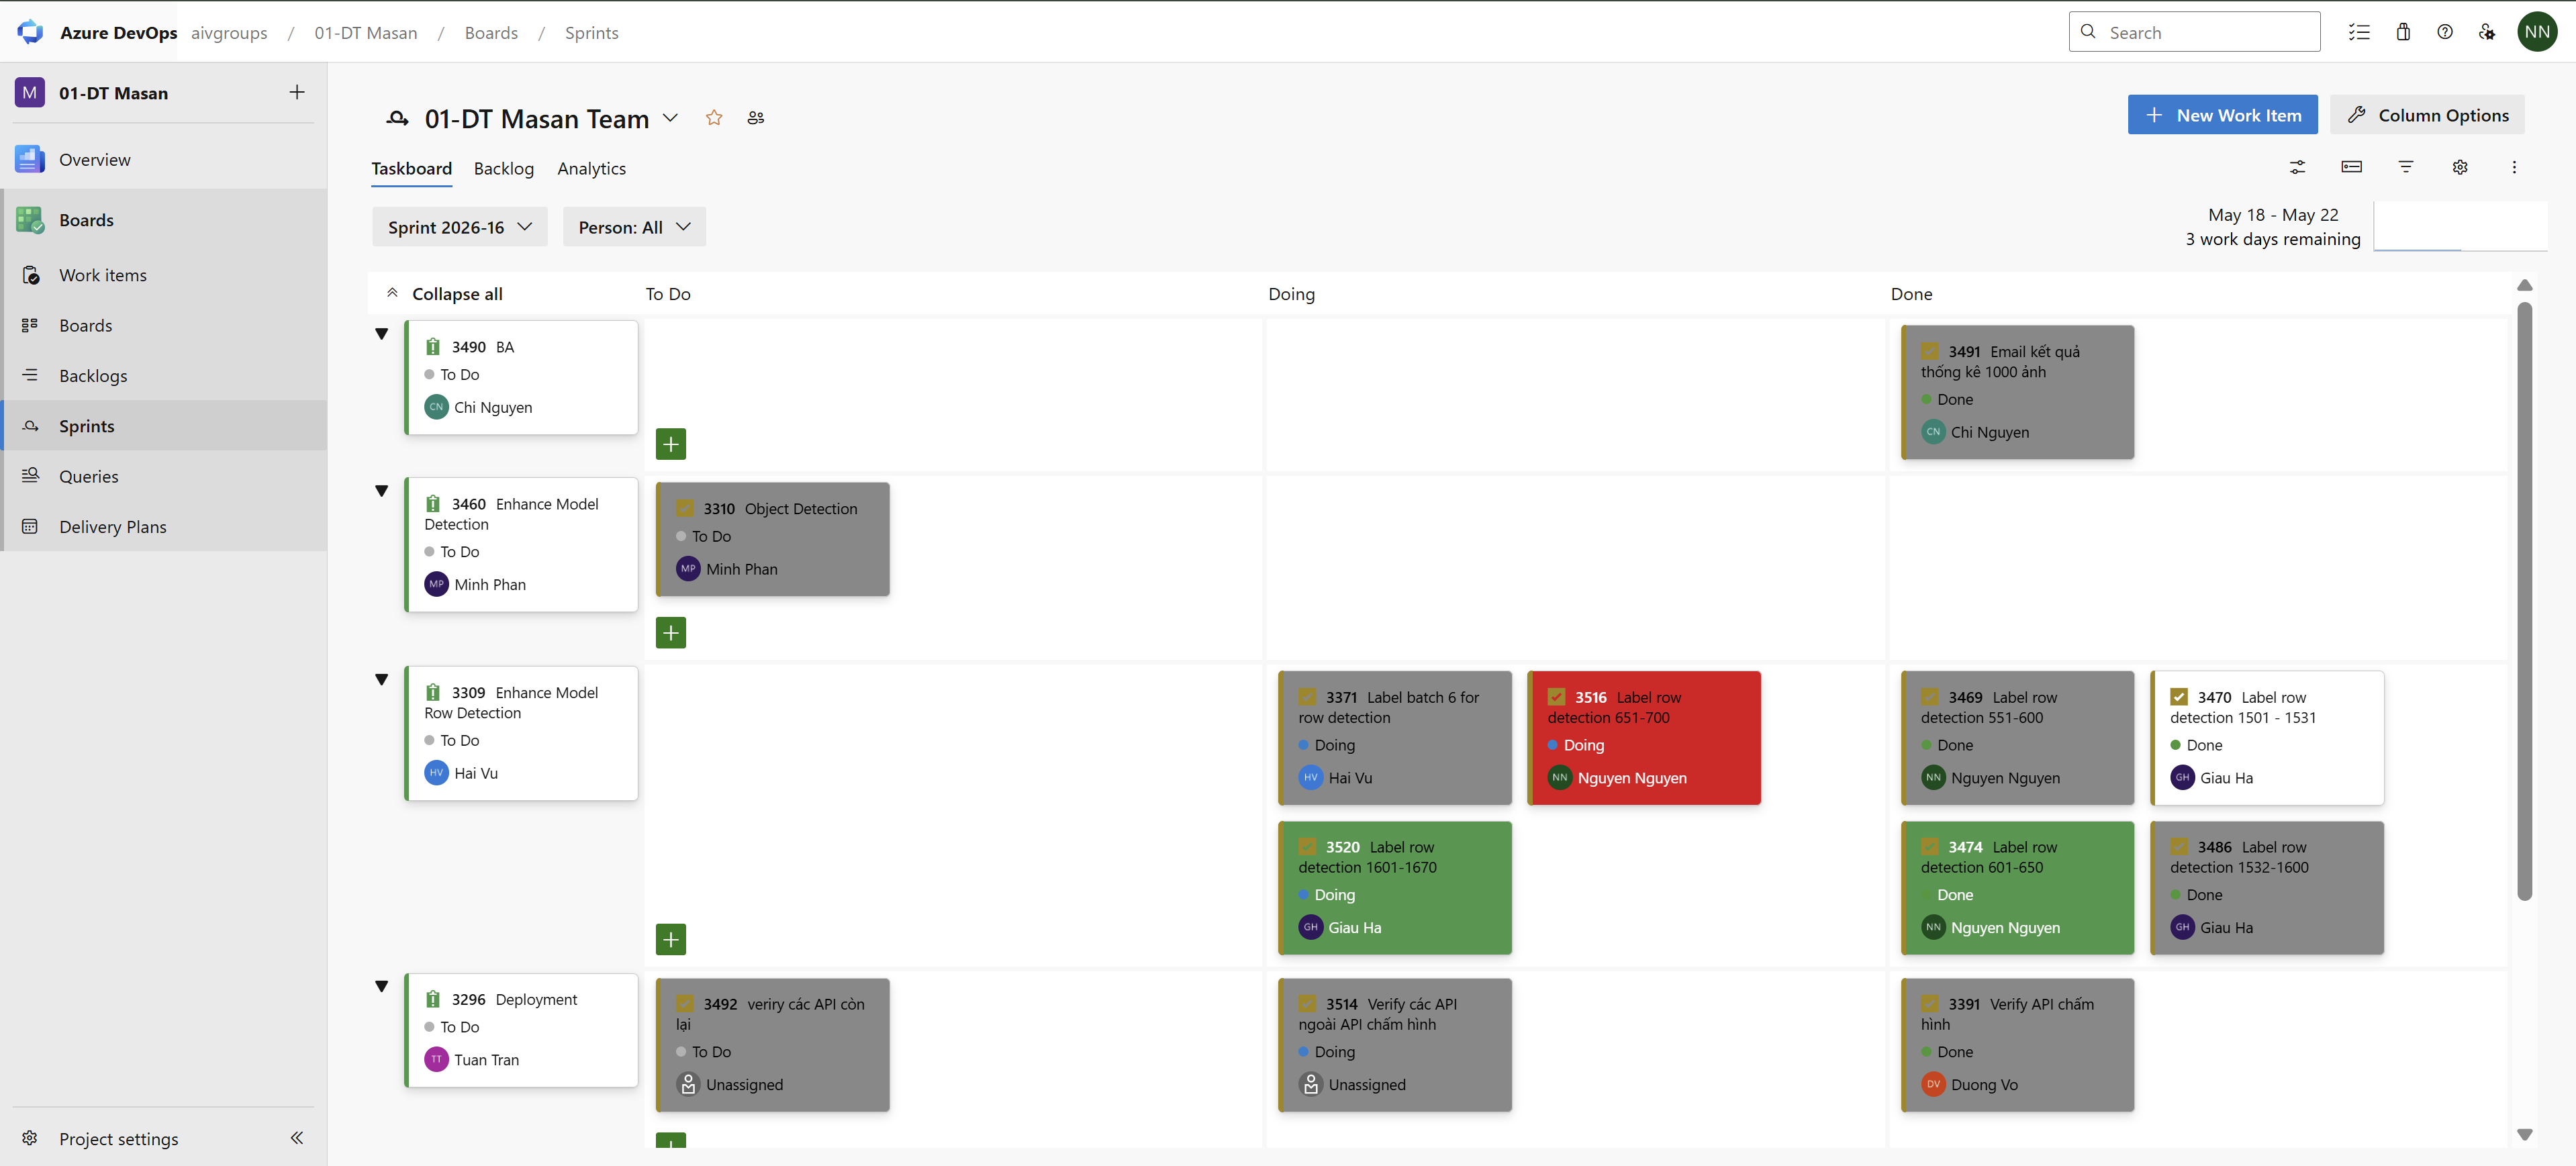
\includegraphics[width=0.95\textwidth]{img/sprint_board.png}
    \caption{Azure DevOps sprint board for the Masan project (Sprint 2026-16).}
    \label{fig:sprintboard}
\end{figure}

\subsection{Meeting Schedule and Facilitation}

Internal meetings followed a fixed weekly structure designed to bookend each work week. A Monday morning session at 10:00 was held at the start of each week to align on sprint goals, assign priorities, and review any incoming requirements or client feedback from the previous week. A Friday afternoon session at 16:30 closed the week with a sprint review — going over completed tasks, updating timelines, and flagging any blockers or scope changes for the following sprint.

In addition to these weekly anchors, daily stand-up meetings were held twice a day at 08:00 and 16:45 on all other weekdays. The morning stand-up opened the day by surfacing blockers and confirming each team member's focus, while the afternoon stand-up provided an end-of-day sync to capture progress, note any issues, and adjust task statuses on the board before the next morning. All meetings were conducted over Microsoft Teams and facilitated internally.

\subsection{Task and Timeline Tracking}

Beyond the Azure DevOps boards, a supplementary Excel tracker was maintained to provide a higher-level view of timelines and ownership across all projects simultaneously. The tracker consolidated key milestones, delivery deadlines, and responsible parties in a format suited to cross-project visibility — particularly useful when reporting status to senior management or when a client requested an overview of the current delivery schedule. An example of the weekly tracking sheet is shown in Figure~\ref{fig:weeklysheet}.

\begin{figure}[h]
    \centering
    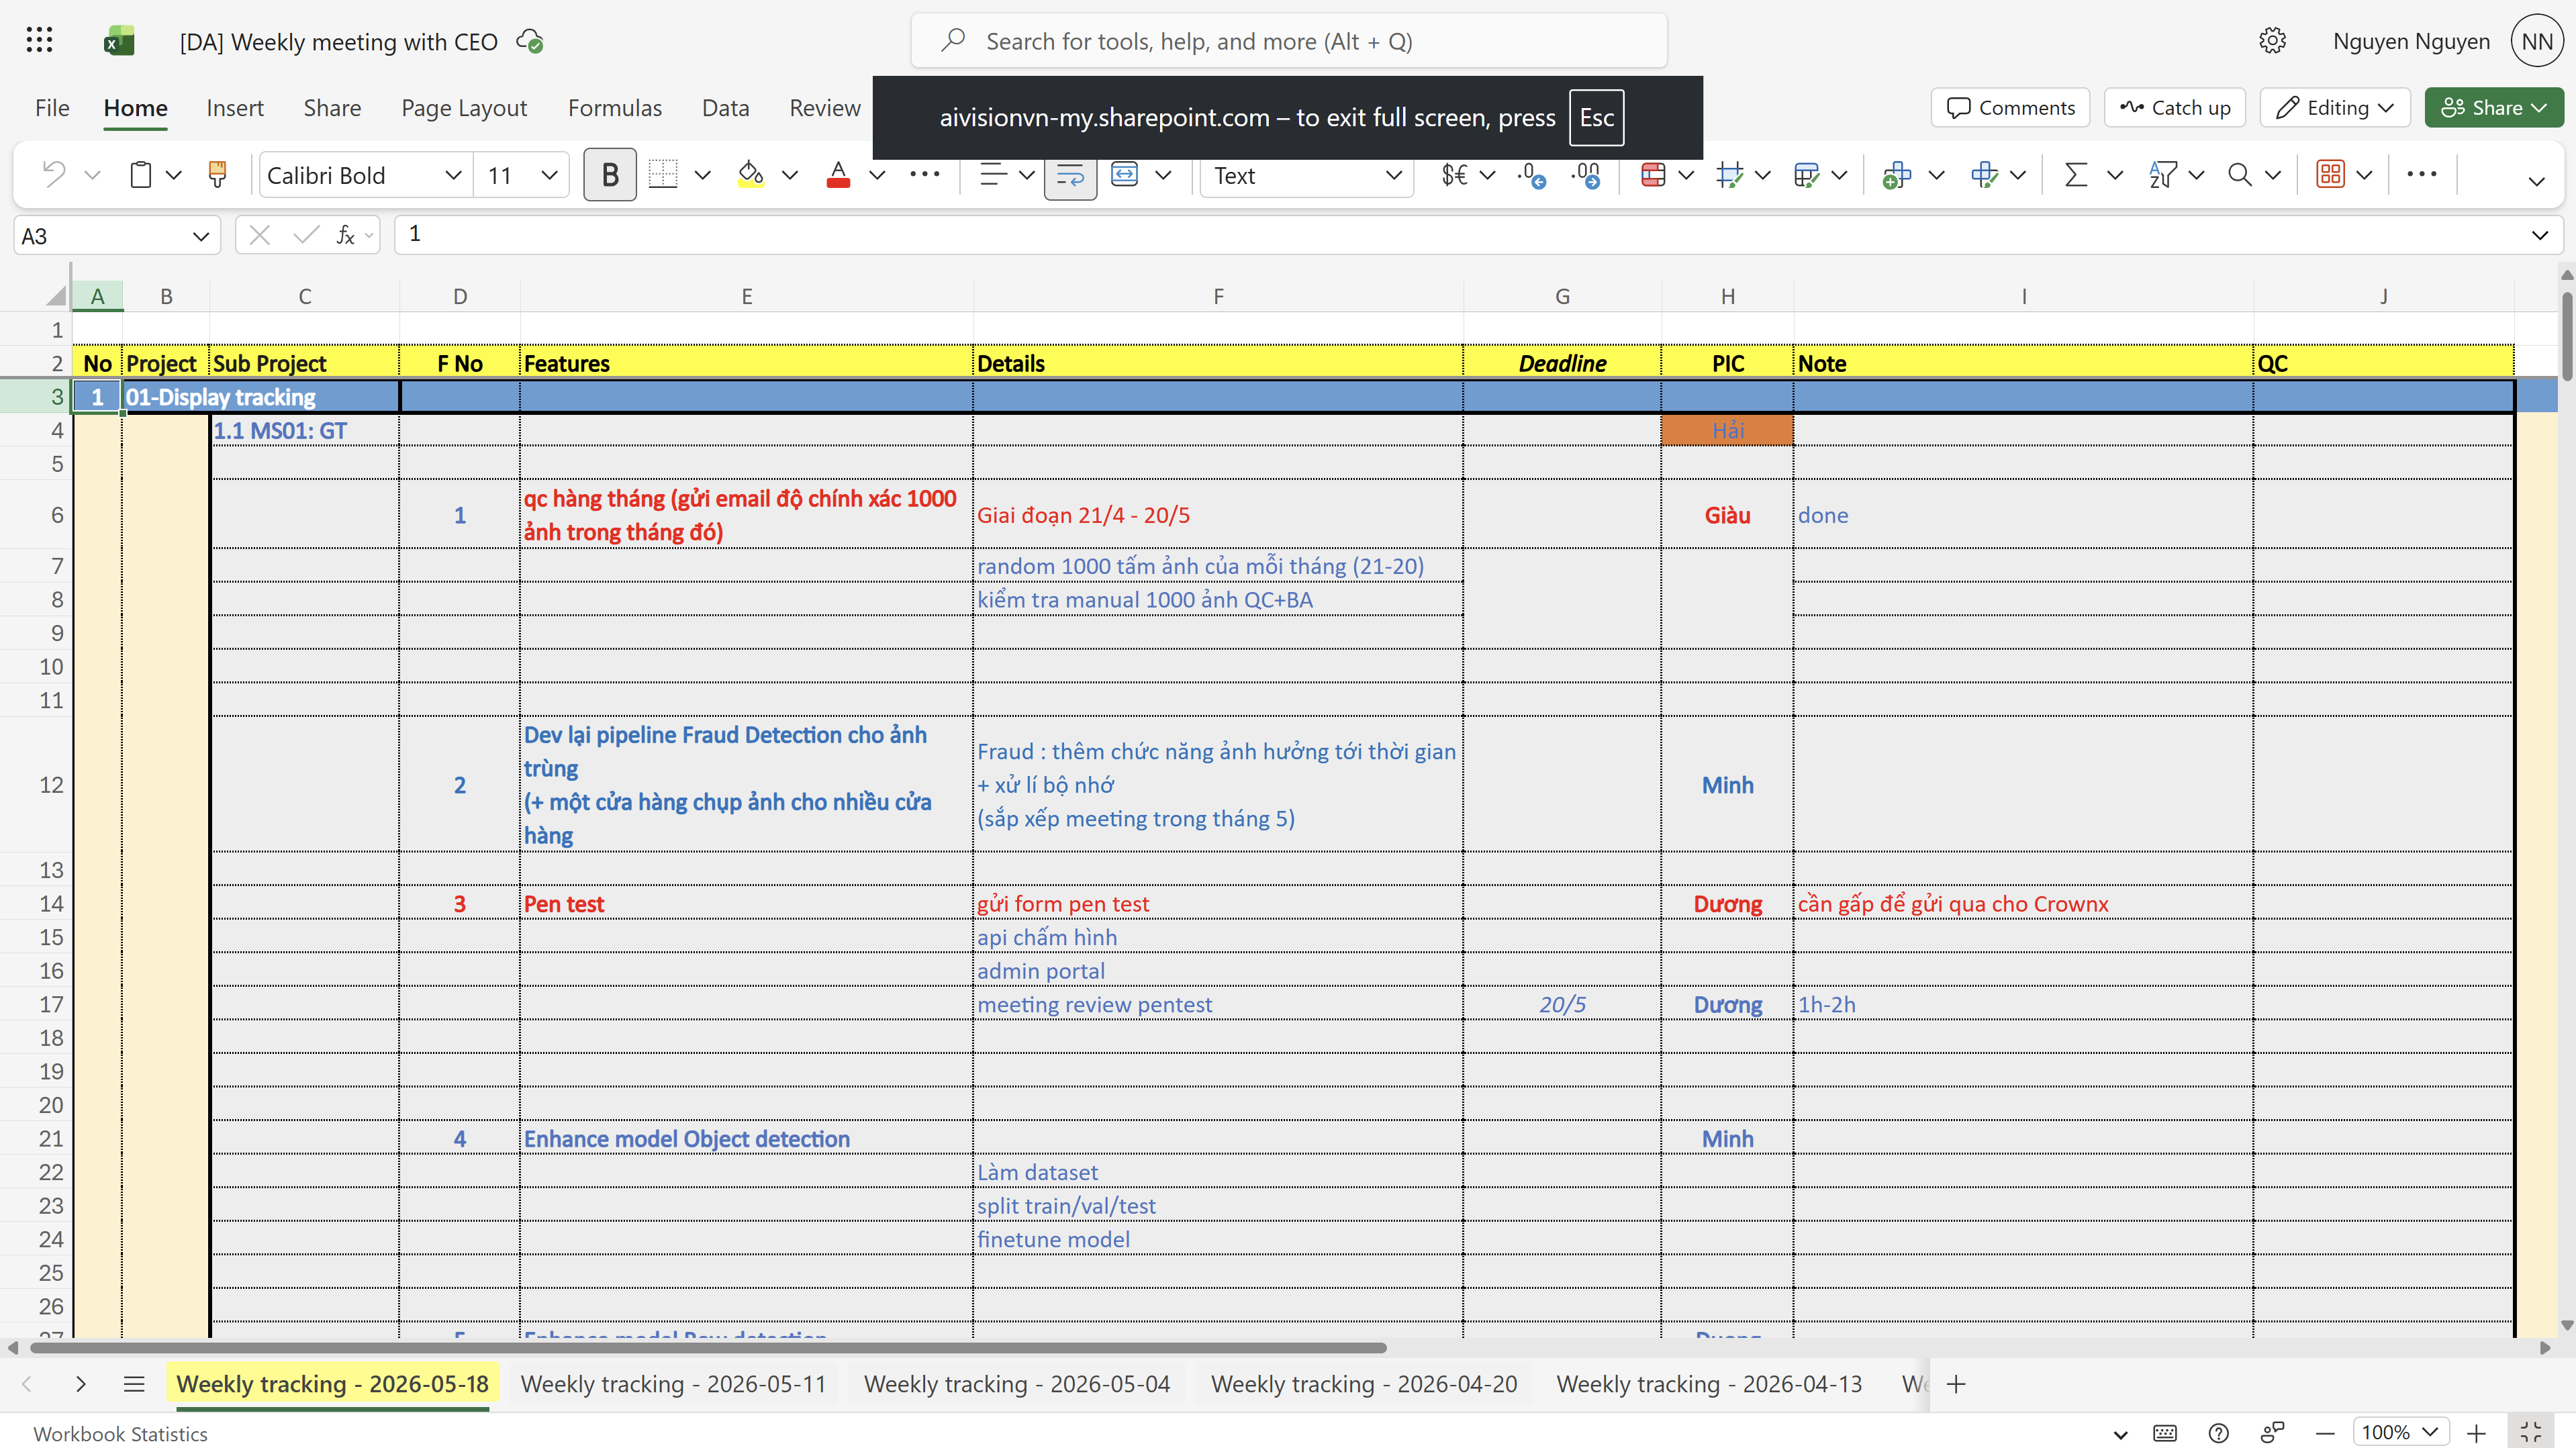
\includegraphics[width=0.95\textwidth]{img/weekly_sheet.png}
    \caption{Weekly task tracking spreadsheet (week of 18 May 2026).}
    \label{fig:weeklysheet}
\end{figure}

\subsection{Client Feedback and Dev Team Coordination}

A significant part of the project management role involved acting as the interface between client feedback and the internal development team. When clients raised issues, change requests, or new requirements in meetings or over email, these were captured, clarified, and translated into actionable tickets on the Azure DevOps board with appropriate priority labels, acceptance criteria, and assigned developers. This ensured that nothing raised in client communication was lost in translation, and that developers received clear, structured work items rather than raw, unfiltered feedback.

\section{Requirements Gathering and Documentation}

\section{Quality Control}
